% This is based on the LLNCS.DEM the demonstration file of
% the LaTeX macro package from Springer-Verlag
% for Lecture Notes in Computer Science,
% version 2.4 for LaTeX2e as of 16. April 2010
%
% See http://www.springer.com/computer/lncs/lncs+authors?SGWID=0-40209-0-0-0
% for the full guidelines.
%

\documentclass{llncs}
\usepackage{graphicx}
\usepackage[usenames, dvipsnames]{color}

\begin{document}

\title{Springer LNCS Example Paper}
%
\titlerunning{Hamiltonian Mechanics}  % abbreviated title (for running head)
%                                     also used for the TOC unless
%                                     \toctitle is used
%
\author{Ivar Ekeland\inst{1} \and Roger Temam\inst{2}
Jeffrey Dean \and David Grove \and Craig Chambers \and Kim~B.~Bruce \and
Elsa Bertino}
%
\authorrunning{Ivar Ekeland et al.} % abbreviated author list (for running head)
%
%%%% list of authors for the TOC (use if author list has to be modified)
\tocauthor{Ivar Ekeland, Roger Temam, Jeffrey Dean, David Grove,
Craig Chambers, Kim B. Bruce, and Elisa Bertino}
%
\institute{Princeton University, Princeton NJ 08544, USA,\\
\email{I.Ekeland@princeton.edu},\\ WWW home page:
\texttt{http://users/\homedir iekeland/web/welcome.html}
\and
Universit\'{e} de Paris-Sud,
Laboratoire d'Analyse Num\'{e}rique, B\^{a}timent 425,\\
F-91405 Orsay Cedex, France}

\maketitle              % typeset the title of the contribution

\begin{abstract}
The abstract should summarize the contents of the paper
using at least 70 and at most 150 words. It will be set in 9-point
font size and be inset 1.0 cm from the right and left margins.
There will be two blank lines before and after the Abstract. \dots
\keywords{computational geometry, graph theory, Hamilton cycles}
\end{abstract}
%
\section{NushellX}
%
%
\subsection{Oxygen isotopes spectra with different interactions}
%
Check .iso file and check if isospin ($\hat{T}^2$) is conserved. usdb Compare with Gustav interaction.
The interactions we choose to compare are: usbd and usda (See Alex article), cceisdpn (Gustav's talk) and sbda ( - Bonn A from Morten - info? Ask Morten => better look at usd (w) to get better comparison from where we started).
Explain difference between usdb and usda (not visible in the energy plots). Maybe look at gamma decay exercise to see the differences.
Compare also with the results of our code.


\begin{figure}[h!]
\centering
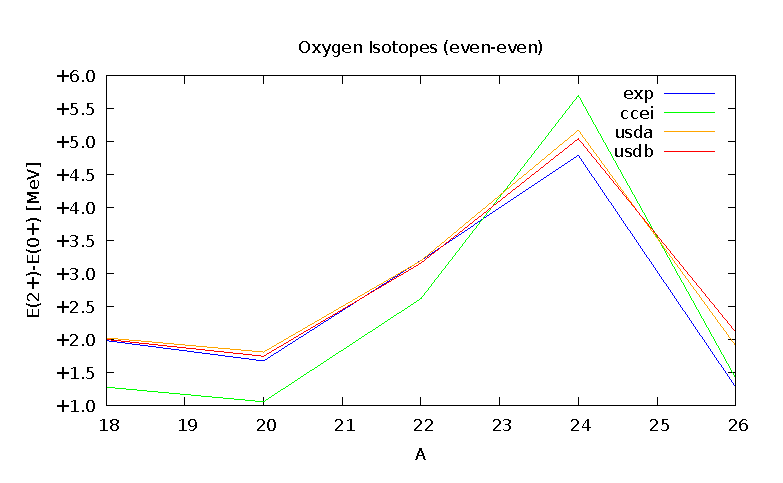
\includegraphics[width=\textwidth]{2+_over_0+.eps}
\caption{Excitation energy of the first $2+$ state in oxygen isotopes (even-even).}
\end{figure}

\begin{figure}[h!]
\centering
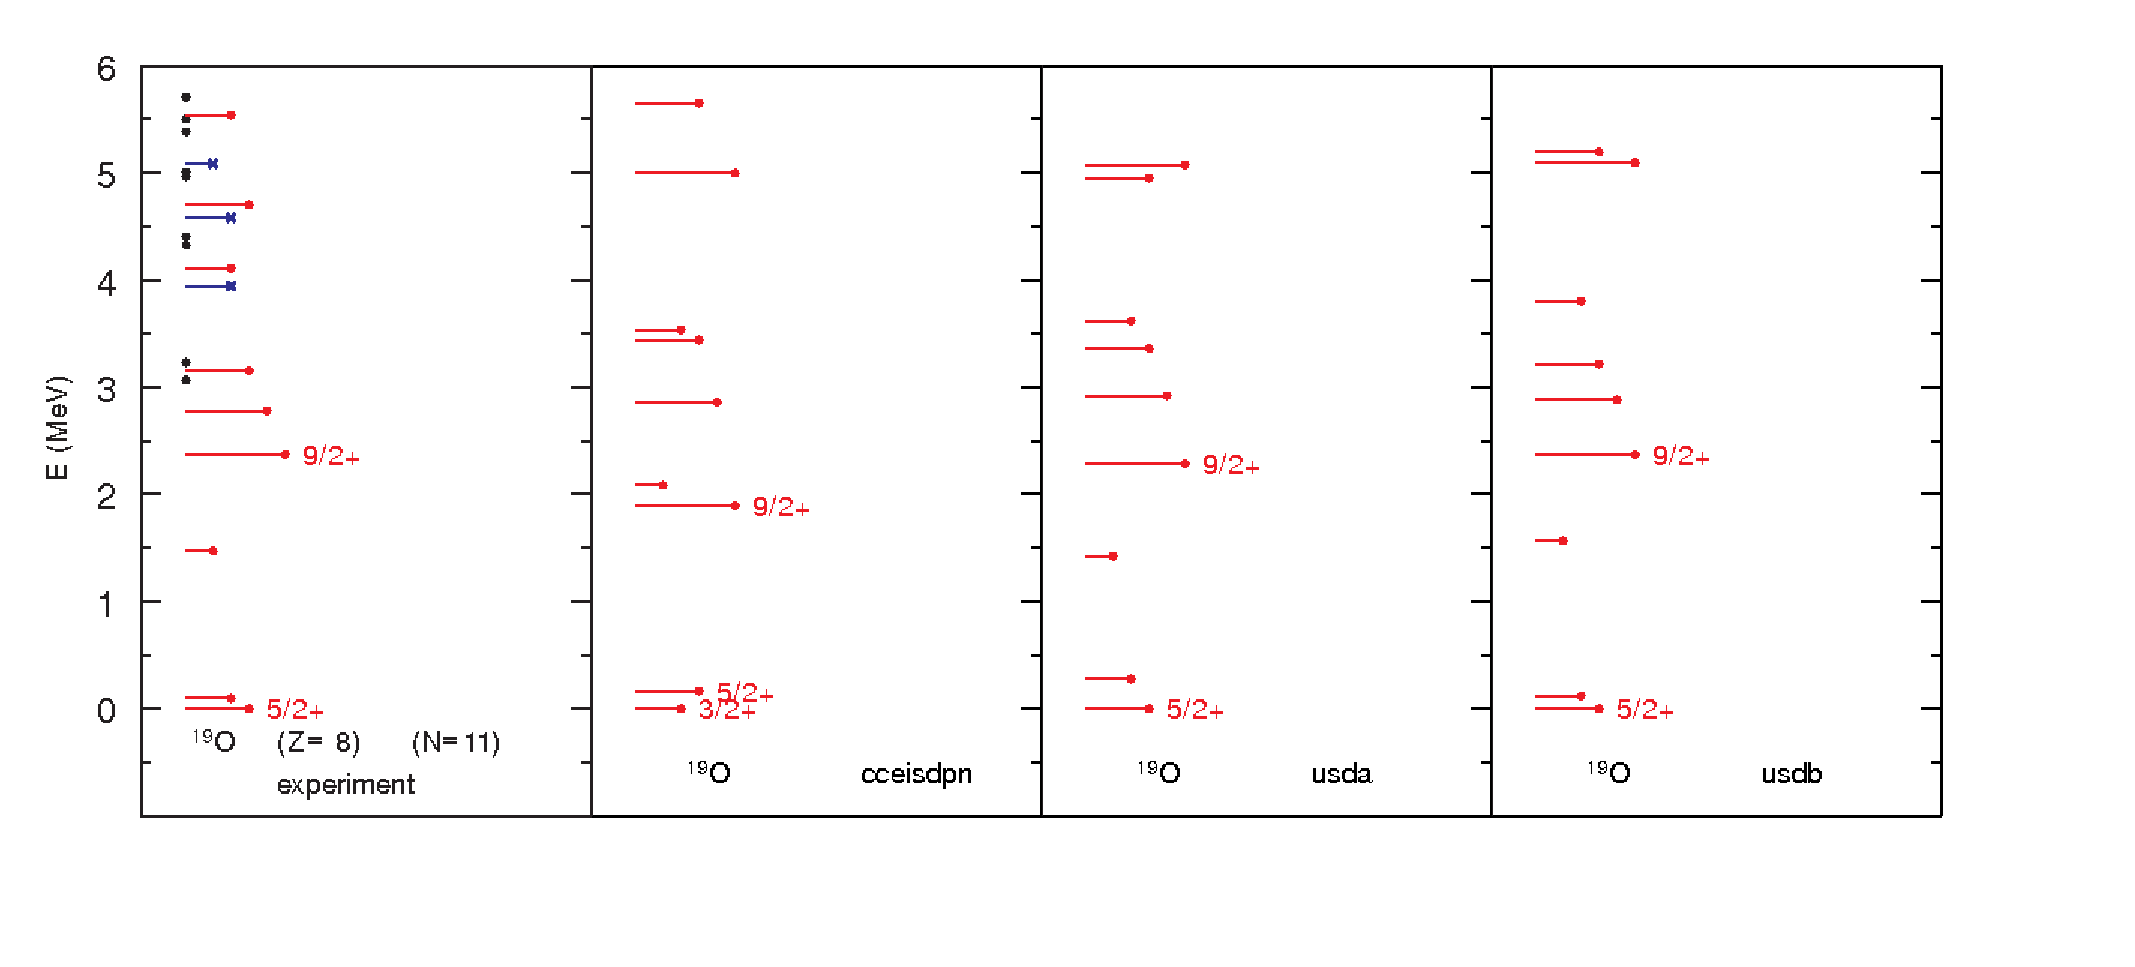
\includegraphics[width=\textwidth]{21O.eps}
\caption{$^{21}$O spectrum with different interactions compared to experiments.}
\end{figure}

%
\subsection{Fermi and Gamow-Teller $\beta$-decay of $^{22}$O.}
%
\begin{table}
\caption{Sum Rules}
\begin{center}
\begin{tabular}{l@{\qquad}l@{\qquad}r@{\qquad}rl}
\hline
\multicolumn{1}{l}{\rule{0pt}{12pt}
                   }&\multicolumn{1}{l}{\rule{0pt}{12pt} sum rule}&\multicolumn{1}{l}{ccei}&\multicolumn{2}{l}{usdb}\\[2pt]
\hline\rule{0pt}{12pt}
sum b(f)            &  $N_i-Z_i=6$   & 5.9993 & 6.0000 &\\
sum qf$\cdot$b(gt)  &  $\ge 3\cdot(N_i-Z_i)=18$  & 6.0346 & 10.0335 &\\[2pt]
\hline
\end{tabular}
\end{center}
\end{table}

With ccei interaction b(f) splits among some states: we have a mixing between closed lying levels, while the usdb interactions gives all the contribution in one single state, which is the isobar analogue of the $^{22}$O \textcolor{red}{(is this true? - Ch. 44 Brown's notes)}.

\begin{table}
\caption{q-value and t$_{1/2}$}
\begin{center}
\begin{tabular}{r@{\qquad}r@{\qquad}r@{\qquad}r@{\qquad}l}
\hline
\multicolumn{1}{l}{\rule{0pt}{12pt}
                   }&\multicolumn{1}{l}{exp}&\multicolumn{1}{l}{ccei}&\multicolumn{2}{l}{usdb}\\[2pt]
\hline\rule{0pt}{12pt}
q-value [MeV]   &     6.489 & 6.847 & 8.437 &\\
t$_{1/2}$ [sec] &     2.25  & 0.478 & 2.620 &\\[2pt]
\hline
\end{tabular}
\end{center}
\end{table}


%
\paragraph{Notes and Comments.}
The results in this section are a
refined version of \cite{clar:eke};
the minimality result of Proposition
14 was the first of its kind.

To understand the nontriviality conditions, such as the one in formula
(\ref{eq:four}), one may think of a one-parameter family
$x_{T}$, $T\in \left(2\pi\omega^{-1}, 2\pi b_{\infty}^{-1}\right)$
of periodic solutions, $x_{T} (0) = x_{T} (T)$,
with $x_{T}$ going away to infinity when $T\to 2\pi \omega^{-1}$,
which is the period of the linearized system at 0.

\paragraph{Notes and Comments.}
The first results on subharmonics were
obtained by Rabinowitz in \cite{rab}, who showed the existence of
infinitely many subharmonics both in the subquadratic and superquadratic
case, with suitable growth conditions on $H'$. Again the duality
approach enabled Clarke and Ekeland in \cite{clar:eke:2} to treat the
same problem in the convex-subquadratic case, with growth conditions on
$H$ only.

Recently, Michalek and Tarantello (see \cite{mich:tar} and \cite{tar})
have obtained lower bound on the number of subharmonics of period $kT$,
based on symmetry considerations and on pinching estimates, as in
Sect.~5.2 of this article.

%
% ---- Bibliography ----
%
\begin{thebibliography}{5}
%
\bibitem {clar:eke}
Clarke, F., Ekeland, I.:
Nonlinear oscillations and
boundary-value problems for Hamiltonian systems.
Arch. Rat. Mech. Anal. 78, 315--333 (1982)

\bibitem {clar:eke:2}
Clarke, F., Ekeland, I.:
Solutions p\'{e}riodiques, du
p\'{e}riode donn\'{e}e, des \'{e}quations hamiltoniennes.
Note CRAS Paris 287, 1013--1015 (1978)

\bibitem {mich:tar}
Michalek, R., Tarantello, G.:
Subharmonic solutions with prescribed minimal
period for nonautonomous Hamiltonian systems.
J. Diff. Eq. 72, 28--55 (1988)

\bibitem {tar}
Tarantello, G.:
Subharmonic solutions for Hamiltonian
systems via a $\bbbz_{p}$ pseudoindex theory.
Annali di Matematica Pura (to appear)

\bibitem {rab}
Rabinowitz, P.:
On subharmonic solutions of a Hamiltonian system.
Comm. Pure Appl. Math. 33, 609--633 (1980)

\end{thebibliography}

\end{document}
